\section{HERM-Schema}
\begin{figure}[ht]
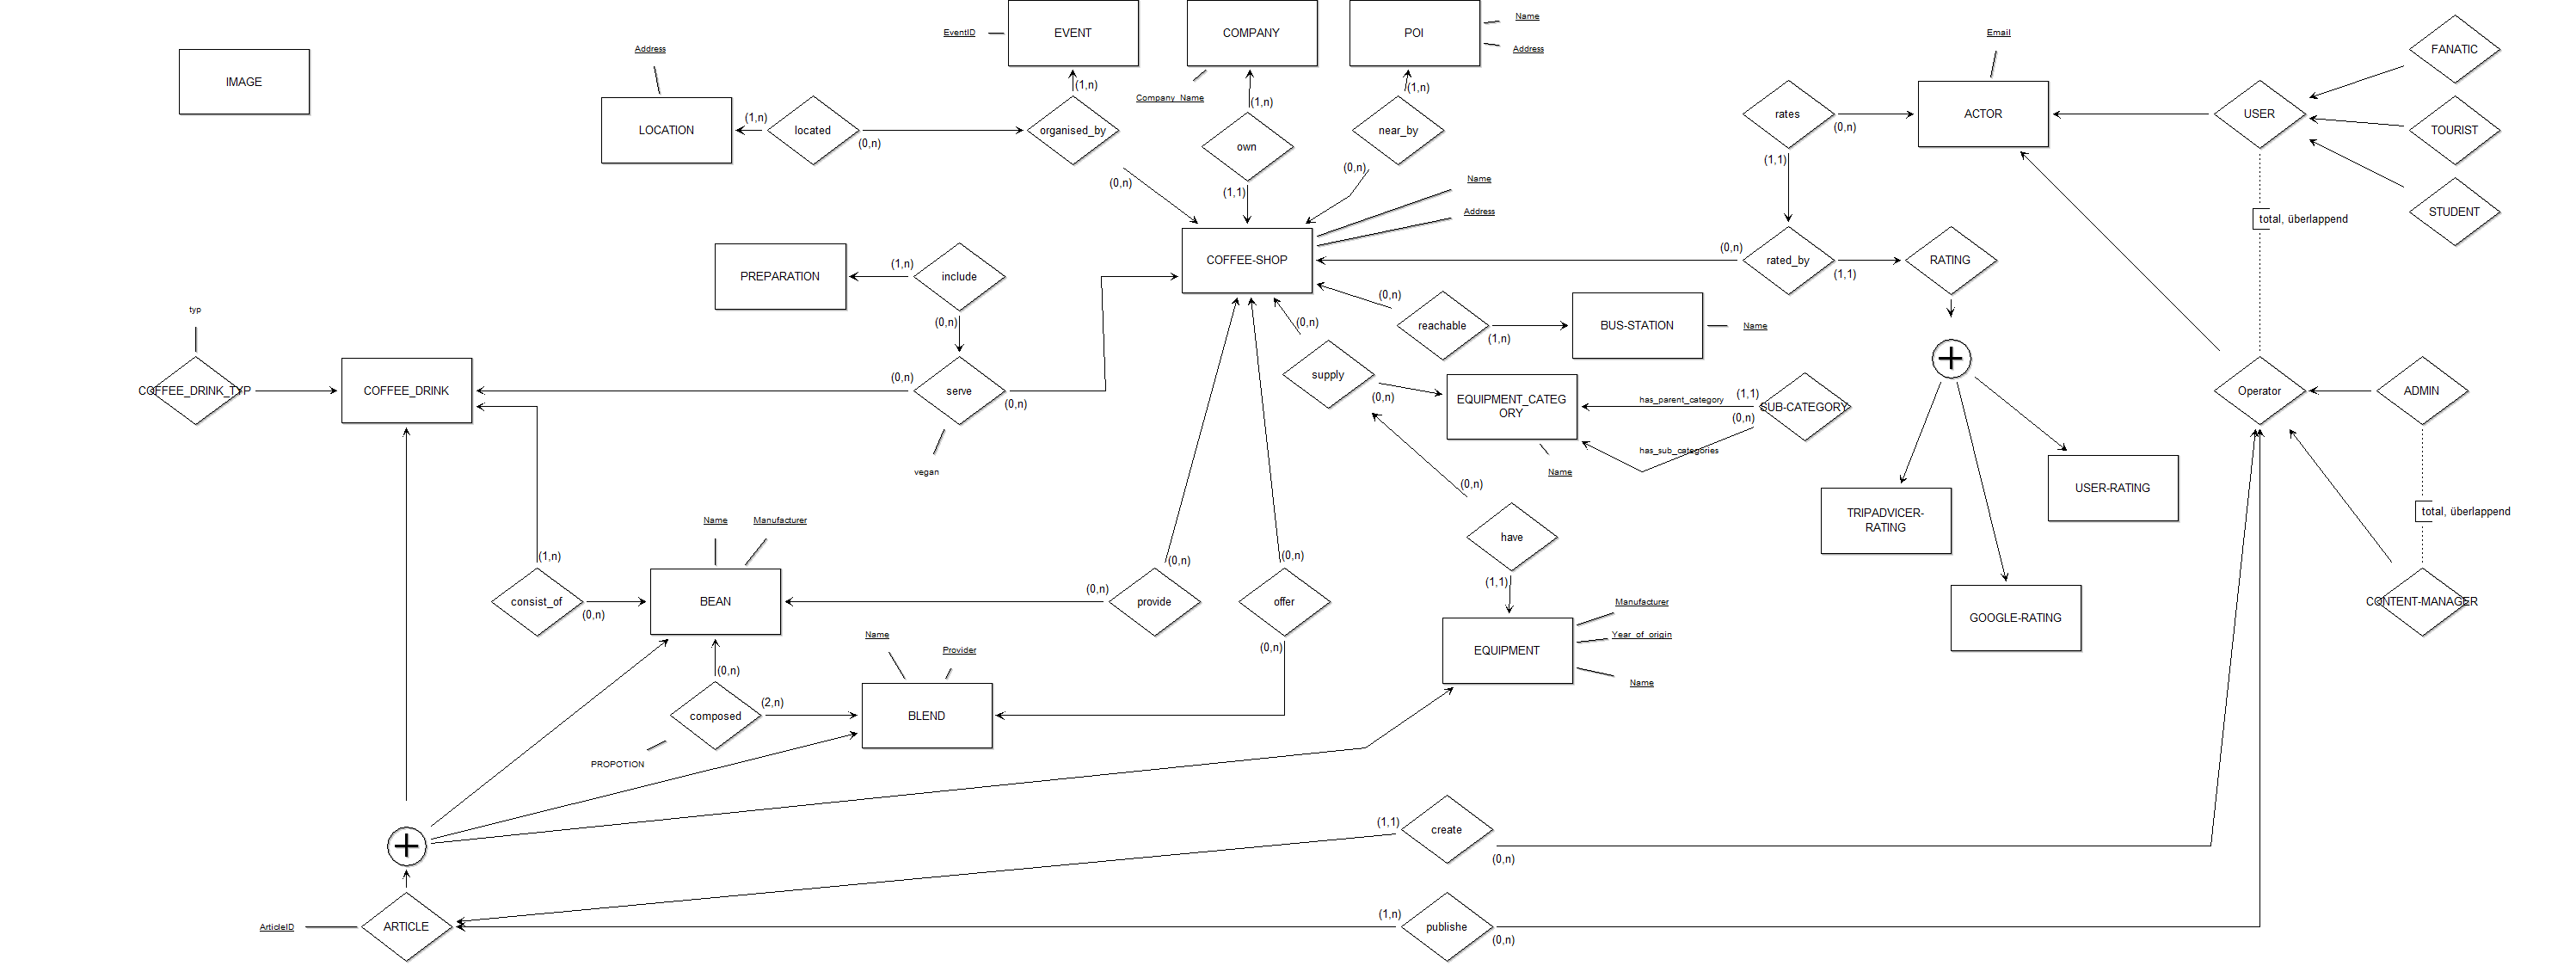
\includegraphics[
    page=1,
    width=\textwidth,
    height=\textheight,
    keepaspectratio
]{Content/HERM/Herm_coffee16_05.png}
\vfill
\caption{Simplify domain model}
\end{figure}
\clearpage
\subsection{HERM-Translation}
\subsubsection{Descripition}
\textbf{Identification}\\\\
The Identification of the entities and relationship is a combination of using natural keys as well as surrogate keys. 
The entity COFFEE-SHOP is the most connected entity in our schema but his natural primary key consist of multiple columns. This cause too much cumbersome workarounds to keep the key natural. For that reason the COFFEE-SHOP entity will have in the implementation another attribute id which will be the new primary key. This new key destroy the 3NF of our schema.\\\\
\textbf{Specialisation}\\\\
All specialisation are total and overlapped. \\\\
\textbf{Higher-Order}\\\\
Located was translate by taken the primary key  of LOCATION as well as the primary keys from the relationship of organised\_by.\\
Rated\_By was translated by\\
Includes was translate by taken the primary key of PREPARATION as well as the primary keys from the relationship of serves.\\
Sells was translated by taken the primary key of EQUIPMENT as well as the primary keys from the relationship supplies.\\\\ 
\textbf{Cluster}\\\\
The ARTICLE cluster with the connection to the following entites: EQUIPMENT, COFFEE\_DRINK, BEAN and BLEND was transformed by using the separation approach where the middle table are collapsed. Seperation was used so that the keys of the connected entites are still the natural one. \\
The RATING cluster with the connection to the following entities: GOOGLE-RATING, USER-RATING, TRIPADVISER-RATING was transformed by using the full participation approach because there is no common key in the entites.\\\\
{ 
\subsubsection{Entities}
(EQUIPMENT(Manufacturer, Year\_of\_origin, Name)(Manufacturer, Year\_of\_origin, Name)),\\
(EVENT(EventID,Start\_Time,Name,Access\_Fee,Description,End\_Time)(EventID)),\\
(COFFEE-SHOP(Name, Address, Outdoor, Fair\_Trade, Disabled\_Friendly, Description, Wlan, Child\_Friendly, Website, Fouding\_Year, Pet\_Friendly, Latte\_Art, Seats, Workstation, Warm food, Cold food, Price\_Class, Franchise)(Name, Address)), \\
(BUS-STATION(Name, Line)(Name,Line)),\\
(COMPANY(Name)(Name)),\\
(BEAN(Name,Provenance,Roast,Grind)(Name,Provenance)),\\
(POI(Name,Address,Description)(Name, Address)), \\
(GOOGLE-RATING()()), \\
(USER-RATING()()), \\
(TRIPADVICER-RATING()()), \\
(BLEND(Name, Provenance, Price\_Range)(Name)), \\
(LOCATION(Address, Description)(Address)), \\
(EQUIPMENT\_CATEGORY(Name)(Name)), \\
(ACTOR(Email,Actor\_Name, Password)(Email)), \\
(PREPARATION(Name, Description, Type)(Name)), \\
(COFFEE\_DRINK(Name, Typ, Description)(Name)), \\
(OPENING-TIME(Close, Open, Weekday)(Close, Open, Weekday)), \\
(MANUFACTURER(Name)(Name)), \\
(RATING(RatingID, RATINGId)(RatingID, RATINGId)),  \\
\subsubsection{Relationships}
(consists\_of(Name, Provenance, Name)(Name, Provenance, Name)),  \\
(serves(Name, Address, Name, vegan)(Name, Address, Name)), \\
(near\_by(Name, Address, Name, Address)(Name, Address, Name, Address)), \\
(reachable(Name, Line, Name, Address)(Name, Line, Name, Address)), \\
(owns(Name, Address, Name)(Name, Address)), \\
(supplies(Name, Name, Address)(Name, Name, Address)), \\
(provides(Name, Address, Name, Provenance)(Name, Address, Name, Provenance)), \\
(offers(Name, Name, Address)(Name, Name, Address)), \\
(organised\_by(Name, Address, EventID)(Name, Address, EventID)), \\
(OPERATOR(Email)(Email)), \\
(SUB-CATEGORY(Name)(Name)), \\
(belongs\_to(Manufacturer, Year\_of\_origin, Name, Name)(Manufacturer, Year\_of\_origin, Name)), \\
(Opens(Name, Address, Close, Open, Weekday)(Name, Address, Close, Open, Weekday)), \\
(produce(Name, Provenance, Name, Product\_Name, Fair\_Trade, Price\_Class)(Name, Provenance, Name)), \\
(includes(Name, Address, Name, Name)(Name, Address, Name, Name)), \\
(composed(Name, Name, Provenance, Name)(Name, Name, Provenance, Name)), \\
(rated\_by(RatingID, RATINGId, Name, Address)(RatingID, RATINGId)), \\
(located(Address, Name, Address, EventID)(Address, Name, Address, EventID)), \\
(sells(Manufacturer, Year\_of\_origin, Name, Name, Name, Address)(Manufacturer, Year\_of\_origin, Name, Name, Name, Address)), \\
(creates(Email, ArticleID)(Email, ArticleID)), \\
(publishes(Email, ArticleID)(Email, ArticleID)), \\
(rates(RatingID, RATINGId, Email)(RatingID, RATINGId))
\subsubsection{Cluster}
(RATINGGOOGLE-RATING(RatingID, RATINGId)(RatingID, RATINGId)), \\
(RATINGUSER-RATING(RatingID, RATINGId)(RatingID, RATINGId)), \\
(RATINGTRIPADVICER-RATING(RatingID, RATINGId)(RatingID, RATINGId)), \\
(ARTICLEEQUIPMENT(ArticleID, Manufacturer, Year\_of\_origin, Name, Exposition, Title)(ArticleID)), \\
(ARTICLEBLEND(ArticleID, Name, Exposition, Title)(ArticleID)), \\
(ARTICLEBEAN(ArticleID, Name, Provenance, Exposition, Title)(ArticleID)), \\
(ARTICLECOFFEE\_DRINK(ArticleID, Name, Exposition, Title)(ArticleID)), \\\\
\subsubsection{Specialisation}
(STUDENT(Email)(Email)), \\
(TOURIST(Email)(Email)), \\
(FANATIC(Email)(Email)), \\
(ADMIN(Email)(Email)), \\
(CONTENT-MANAGER(Email)(Email)), \\
(USER(Email)(Email)), \\
 } 
\subsubsection{Integrity Constraints}
EVENT[EventID]\\$\subseteq$organised\_by[EventID]\\
BUS-STATION[Name,  Line]\\$\subseteq$reachable[Name,  Line]\\
COMPANY[Name]$\subseteq$owns[Name]\\
BEAN[Name,  Provenance]$\subseteq$produce[Name,  Provenance]\\
POI[Name,  Address]$\subseteq$near\_by[Name,  Address]\\
LOCATION[Address]$\subseteq$located[Address]\\
COFFEE\_DRINK[Name]$\subseteq$consists\_of[Name]\\
Manufacutrer[Name]$\subseteq$produce[Name]\\
USER[Email]$\subseteq$ACTOR[Email]\\
consists\_of[Name,  Provenance]$\subseteq$BEAN[Name,  Provenance]\\
consists\_of[Name]$\subseteq$COFFEE\_DRINK[Name]\\
serves[Name,  Address]$\subseteq$COFFEE-SHOP[Name,  Address]\\
serves[Name]$\subseteq$COFFEE\_DRINK[Name]\\
near\_by[Name,  Address]$\subseteq$COFFEE-SHOP[Name,  Address]\\
near\_by[Name,  Address]$\subseteq$POI[Name,  Address]\\
reachable[Name,  Line]$\subseteq$BUS-STATION[Name,  Line]\\
reachable[Name,  Address]$\subseteq$COFFEE-SHOP[Name,  Address]\\
owns[Name,  Address]$\subseteq$COFFEE-SHOP[Name,  Address]\\
owns[Name]$\subseteq$COMPANY[Name]\\
supplies[Name]$\subseteq$EQUIPMENT\_CATEGORY[Name]\\
supplies[Name,  Address]$\subseteq$COFFEE-SHOP[Name,  Address]\\
provides[Name,  Address]$\subseteq$COFFEE-SHOP[Name,  Address]\\
provides[Name,  Provenance]$\subseteq$BEAN[Name,  Provenance]\\
offers[Name]$\subseteq$BLEND[Name]\\
offers[Name,  Address]$\subseteq$COFFEE-SHOP[Name,  Address]\\
organised\_by[Name,  Address]$\subseteq$COFFEE-SHOP[Name,  Address]\\
organised\_by[EventID]$\subseteq$EVENT[EventID]\\
OPERATOR[Email]$\subseteq$ACTOR[Email]\\
SUB-CATEGORY[Name]$\subseteq$EQUIPMENT\_CATEGORY[Name]\\
SUB-CATEGORY[Name]$\subseteq$EQUIPMENT\_CATEGORY[Name]\\
SUB-CATEGORY[]$\subseteq$EQUIPMENT\_CATEGORY[]\\
belongs\_to[Name]$\subseteq$EQUIPMENT\_CATEGORY[Name]\\
belongs\_to[Manufacturer,  Year\_of\_origin,  Name]$\subseteq$EQUIPMENT[Manufacturer,  Year\_of\_origin,  Name]\\
Opens[Name,  Address]$\subseteq$COFFEE-SHOP[Name,  Address]\\
Opens[Close,  Open,  Weekday]$\subseteq$Opening-Time[Close,  Open,  Weekday]\\
produce[Name,  Provenance]$\subseteq$BEAN[Name,  Provenance]\\
produce[Name]$\subseteq$Manufacutrer[Name]\\
includes[Name,  Address,  Name]$\subseteq$serves[Name,  Address,  Name]\\
includes[Name]$\subseteq$PREPARATION[Name]\\
composed[Name]$\subseteq$BLEND[Name]\\
composed[Name,  Provenance,  Name]$\subseteq$produce[Name,  Provenance,  Name]\\
rated\_by[Name,  Address]$\subseteq$COFFEE-SHOP[Name,  Address]\\
rated\_by[RatingID,  RATINGId]$\subseteq$RATING[RatingID,  RATINGId]\\
located[Address]$\subseteq$LOCATION[Address]\\
located[Name,  Address,  EventID]$\subseteq$organised\_by[Name,  Address,  EventID]\\
sells[Manufacturer,  Year\_of\_origin,  Name]$\subseteq$EQUIPMENT[Manufacturer,  Year\_of\_origin,  Name]\\
sells[Name,  Name,  Address]$\subseteq$supplies[Name,  Name,  Address]\\
STUDENT[Email]$\subseteq$USER[Email]\\
TOURIST[Email]$\subseteq$USER[Email]\\
FANATIC[Email]$\subseteq$USER[Email]\\
ADMIN[Email]$\subseteq$OPERATOR[Email]\\
CONTENT-MANAGER[Email]$\subseteq$OPERATOR[Email]\\
creates[Email]$\subseteq$OPERATOR[Email]\\
creates[ArticleID]$\subseteq$ARTICLEEQUIPMENT[ArticleID]\\
creates[ArticleID]$\subseteq$ARTICLEBLEND[ArticleID]\\
creates[ArticleID]$\subseteq$ARTICLEBEAN[ArticleID]\\
creates[ArticleID]$\subseteq$ARTICLECOFFEE\_DRINK[ArticleID]\\
publishes[Email]$\subseteq$OPERATOR[Email]\\
publishes[ArticleID]$\subseteq$ARTICLEEQUIPMENT[ArticleID]\\
publishes[ArticleID]$\subseteq$ARTICLEBLEND[ArticleID]\\
publishes[ArticleID]$\subseteq$ARTICLEBEAN[ArticleID]\\
publishes[ArticleID]$\subseteq$ARTICLECOFFEE\_DRINK[ArticleID]\\
rates[RatingID,  RATINGId]$\subseteq$rated\_by[RatingID,  RATINGId]\\
rates[Email]$\subseteq$ACTOR[Email]\\
ARTICLEEQUIPMENT[ArticleID]\\||ARTICLEBLEND[ArticleID]\\||ARTICLEBEAN[ArticleID]\\||ARTICLECOFFEE\_DRINK[ArticleID]\\
\subsubsection{Data Type}
EQUIPMENT.Manufacturer::VARCHAR(n)
EQUIPMENT.Year\_of\_origin::VARCHAR(n)
EQUIPMENT.Name::VARCHAR(n)\\
EVENT.EventID::INTEGER\\
EVENT.Start\_Time::INTEGER\\
EVENT.Name::VARCHAR(n)\\
EVENT.Access\_Fee::INTEGER\\
EVENT.Description::VARCHAR(n)\\
EVENT.End\_Time::TIME
COFFEE-SHOP.Name::VARCHAR(n)\\
COFFEE-SHOP.Address::VARCHAR(n)\\
COFFEE-SHOP.Outdoor::BOOLEAN\\
COFFEE-SHOP.Fair\_Trade::BOOLEAN\\
COFFEE-SHOP.Disabled\_Friendly::BOOLEAN\\
COFFEE-SHOP.Description::VARCHAR(n)\\
COFFEE-SHOP.Wlan::BOOLEAN\\
COFFEE-SHOP.Child\_Friendly::BOOLEAN\\
COFFEE-SHOP.Website::VARCHAR(n)\\
COFFEE-SHOP.Fouding\_Year::INTEGER\\
COFFEE-SHOP.Pet\_Friendly::BOOLEAN\\
COFFEE-SHOP.Latte\_Art::VARCHAR(n)\\
COFFEE-SHOP.Seats::VARCHAR(n)\\
COFFEE-SHOP.Workstation::BOOLEAN\\
COFFEE-SHOP.Food::VARCHAR(n)\\
COFFEE-SHOP.Price\_Class::VARCHAR(n)\\
COFFEE-SHOP.Franchise::BOOLEAN\\
BUS-STATION.Name::VARCHAR(n)\\
BUS-STATION.Line::VARCHAR(n)\\
COMPANY.Name::VARCHAR(n)\\
BEAN.Name::VARCHAR(n)\\
BEAN.Provenance::VARCHAR(n)\\
BEAN.Type::VARCHAR(n)\\
POI.Name::VARCHAR(n)\\
POI.Address::VARCHAR(n)\\
POI.Description::CHARACTER(n)\\
BLEND.Name::VARCHAR(n)\\
BLEND.Provenance::VARCHAR(n)\\
BLEND.Price\_Range::INTEGER\\
LOCATION.Address::VARCHAR(n)\\
LOCATION.Description::VARCHAR(n)\\
EQUIPMENT\_CATEGORY.Name::VARCHAR(n)\\
ACTOR.Email::VARCHAR(n)\\
ACTOR.Actor\_Name::VARCHAR(n)\\
ACTOR.Password::VARCHAR(n)\\
PREPARATION.Description::VARCHAR(n)\\
PREPARATION.Type::VARCHAR(n)\\
PREPARATION.Name::VARCHAR(n)\\
COFFEE\_DRINK.Typ::VARCHAR(n)\\
COFFEE\_DRINK.Name::VARCHAR(n)\\
COFFEE\_DRINK.Description::VARCHAR(n)\\
Opening-Time.Close::INTEGER\\
Opening-Time.Open::INTEGER\\
Opening-Time.Weekday::VARCHAR(n)\\
Manufacutrer.Name::VARCHAR(n)\\
USER.Email::VARCHAR(n)\\
RATING.RatingID::INTEGER\\
RATING.RATINGId::INTEGER\\
consists\_of.Name::VARCHAR(n)\\
consists\_of.Provenance::VARCHAR(n)\\
consists\_of.Name::VARCHAR(n)\\
serves.vegan::BOOLEAN\\
serves.Name::VARCHAR(n)\\
serves.Address::VARCHAR(n)\\
serves.Name::VARCHAR(n)\\
near\_by.Name::VARCHAR(n)\\
near\_by.Address::VARCHAR(n)\\
near\_by.Name::VARCHAR(n)\\
near\_by.Address::VARCHAR(n)\\
reachable.Name::VARCHAR(n)\\
reachable.Line::VARCHAR(n)\\
reachable.Name::VARCHAR(n)\\
reachable.Address::VARCHAR(n)\\
owns.Name::VARCHAR(n)\\
owns.Address::VARCHAR(n)\\
owns.Name::VARCHAR(n)\\
supplies.Name::VARCHAR(n)\\
supplies.Name::VARCHAR(n)\\
supplies.Address::VARCHAR(n)\\
provides.Name::VARCHAR(n)\\
provides.Address::VARCHAR(n)\\
provides.Name::VARCHAR(n)\\
provides.Provenance::VARCHAR(n)\\
offers.Name::VARCHAR(n)\\
offers.Name::VARCHAR(n)\\
offers.Address::VARCHAR(n)\\
organised\_by.Name::VARCHAR(n)\\
organised\_by.Address::VARCHAR(n)\\
organised\_by.EventID::INTEGER\\
OPERATOR.Email::VARCHAR(n)\\
SUB-CATEGORY.Name::CHAR
belongs\_to.Manufacturer::VARCHAR(n)\\
belongs\_to.Year\_of\_origin::VARCHAR(n)\\
belongs\_to.Name::VARCHAR(n)\\
belongs\_to.Name::VARCHAR(n)\\
Opens.Name::VARCHAR(n)\\
Opens.Address::VARCHAR(n)\\
Opens.Close::INTEGER\\
Opens.Open::INTEGER\\
Opens.Weekday::VARCHAR(n)\\
produce.Product\_Name::VARCHAR(n)\\
produce.Fair\_Trade::BOOLEAN\\
produce.Price\_Class::CHARACTER(n)\\
produce.Name::VARCHAR(n)\\
produce.Provenance::VARCHAR(n)\\
produce.Name::VARCHAR(n)\\
RATINGGOOGLE-RATING.RatingID::INTEGER\\
RATINGGOOGLE-RATING.RATINGId::INTEGER\\
RATINGUSER-RATING.RatingID::INTEGER\\
RATINGUSER-RATING.RATINGId::INTEGER\\
RATINGTRIPADVICER-RATING.RatingID::INTEGER\\
RATINGTRIPADVICER-RATING.RATINGId::INTEGER\\
ARTICLEEQUIPMENT.ArticleID::INTEGER\\
ARTICLEEQUIPMENT.Manufacturer::VARCHAR(n)\\
ARTICLEEQUIPMENT.Year\_of\_origin::VARCHAR(n)\\
ARTICLEEQUIPMENT.Name::VARCHAR(n)\\
ARTICLEEQUIPMENT.Exposition::CHARACTER(n)\\
ARTICLEEQUIPMENT.Title::VARCHAR(n)\\
ARTICLEBLEND.ArticleID::INTEGER\\
ARTICLEBLEND.Name::VARCHAR(n)\\
ARTICLEBLEND.Exposition::CHARACTER(n)\\
ARTICLEBLEND.Title::VARCHAR(n)\\
ARTICLEBEAN.ArticleID::INTEGER\\
ARTICLEBEAN.Name::VARCHAR(n)\\
ARTICLEBEAN.Provenance::VARCHAR(n)\\
ARTICLEBEAN.Exposition::CHARACTER(n)\\
ARTICLEBEAN.Title::VARCHAR(n)\\
ARTICLECOFFEE\_DRINK.ArticleID::INTEGER\\
ARTICLECOFFEE\_DRINK.Name::VARCHAR(n)\\
ARTICLECOFFEE\_DRINK.Exposition::CHARACTER(n)\\
ARTICLECOFFEE\_DRINK.Title::VARCHAR(n)\\
includes.Name::VARCHAR(n)\\
includes.Address::VARCHAR(n)\\
includes.Name::VARCHAR(n)\\
includes.Name::VARCHAR(n)\\
composed.Name::VARCHAR(n)\\
composed.Name::VARCHAR(n)\\
composed.Provenance::VARCHAR(n)\\
composed.Name::VARCHAR(n)\\
rated\_by.RatingID::INTEGER\\
rated\_by.RATINGId::INTEGER\\
rated\_by.Name::VARCHAR(n)\\
rated\_by.Address::VARCHAR(n)\\
located.Address::VARCHAR(n)\\
located.Name::VARCHAR(n)\\
located.Address::VARCHAR(n)\\
located.EventID::INTEGER\\
sells.Manufacturer::VARCHAR(n)\\
sells.Year\_of\_origin::VARCHAR(n)\\
sells.Name::VARCHAR(n)\\
sells.Name::VARCHAR(n)\\
sells.Name::VARCHAR(n)\\
sells.Address::VARCHAR(n)\\
STUDENT.Email::VARCHAR(n)\\
TOURIST.Email::VARCHAR(n)\\
FANATIC.Email::VARCHAR(n)\\
ADMIN.Email::VARCHAR(n)\\
CONTENT-MANAGER.Email::VARCHAR(n)\\
creates.Email::VARCHAR(n)\\
creates.ArticleID::INTEGER\\
publishes.Email::VARCHAR(n)\\
publishes.ArticleID::INTEGER\\
rates.RatingID::INTEGER\\
rates.RATINGId::INTEGER\\
rates.Email::VARCHAR(n)\\

\subsection{Constraints Handling}
Referential constraints are enforced through the database management system by adding constraint to the tables which have the corresponding references. The majority of the referential constraints are foreign keys constraints.\\  Integrity of concrete input of some tables are enforces through checks.\\
\newpage